\section{Related Work}

\begin{figure}[t]
    \centering
    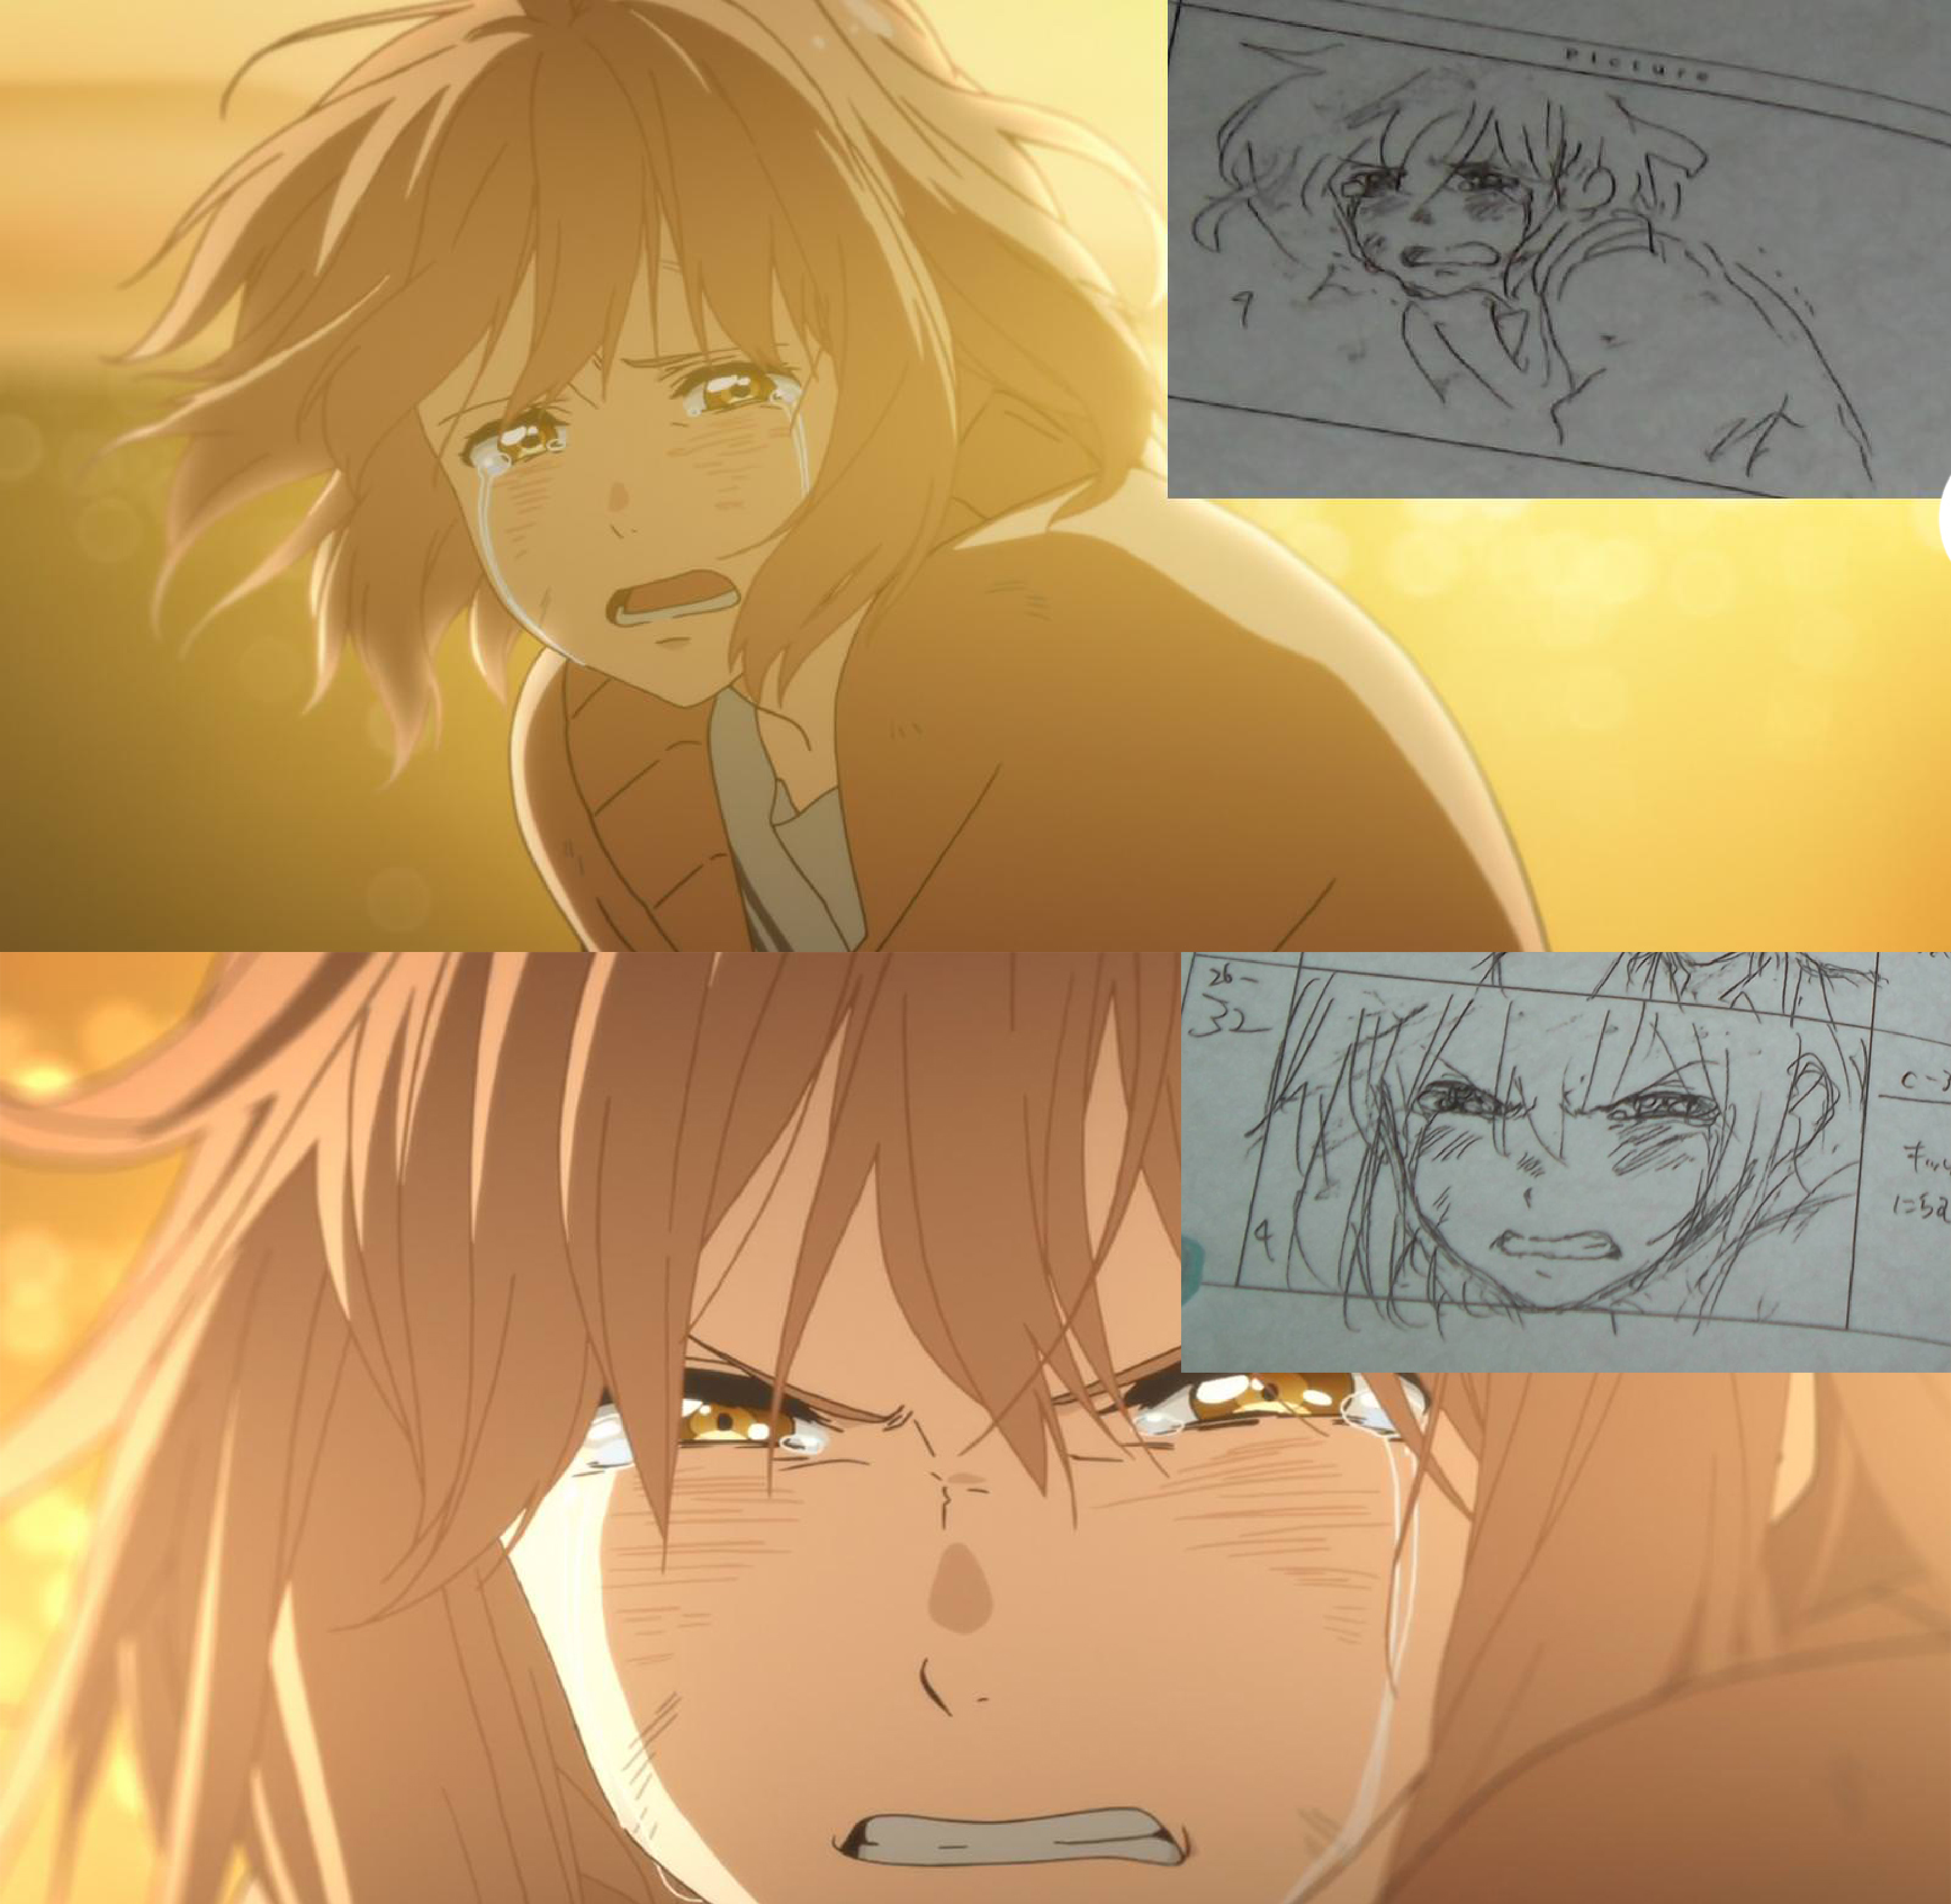
\includegraphics[width=1\linewidth]{img/relatedwork/kyoukai_ishidate.pdf} \\
    \caption{\textbf{Top right:} Storyboard version of scenes in Kyoukai no Kanata (Beyond the Boundary) by Ishidate Taichi. \textbf{Main:} Actual scenes in anime output of storyboards~\cite{kyoAniDirectionTaichi}.}
    \vspace{-15pt}
    \label{fig:kyoukai_ishidate}
\end{figure}

Kyoto Animation's production process. Kyoto Animation is widely-known for its high attention to detail and quality animation that is based on a number of factors: direction~\cite{kyoAniDirectionTaichi, kyoAniDirectionFujita, kyoAniDirectionYamada}, employee management~\cite{kyoAniEmployeeMgmt, kyoAniCulture}, and training process~\cite{kyoAniTour, kyoAniSchool}. Their processes focus on improving full-time employees' abilities into animators who can both draw and direct, which is highly unconventional given the current industry's trend of outsourcing and dispatch hiring for keyin animation. Focusing on the direction process, the aim of storyboard artists and directors at Kyoto Animation is to more or less create a clear picture of their vision for animators to simply draw in, thereby focusing simply on improving the animation aspect~\cite{principlesOfAnimation} and not think much about how to draw and animate that vision. This applies a concept similar to Computer Science's widely-known Single Responsibility Principle~\cite{singleResponsibilityPrinciple}, which manages complexity by having modules focus on a single function. This has been applied to the pipeline in this paper and improved using the said 3D modeling and motion capture processes.\\\\

\begin{figure}[t]
    \centering
    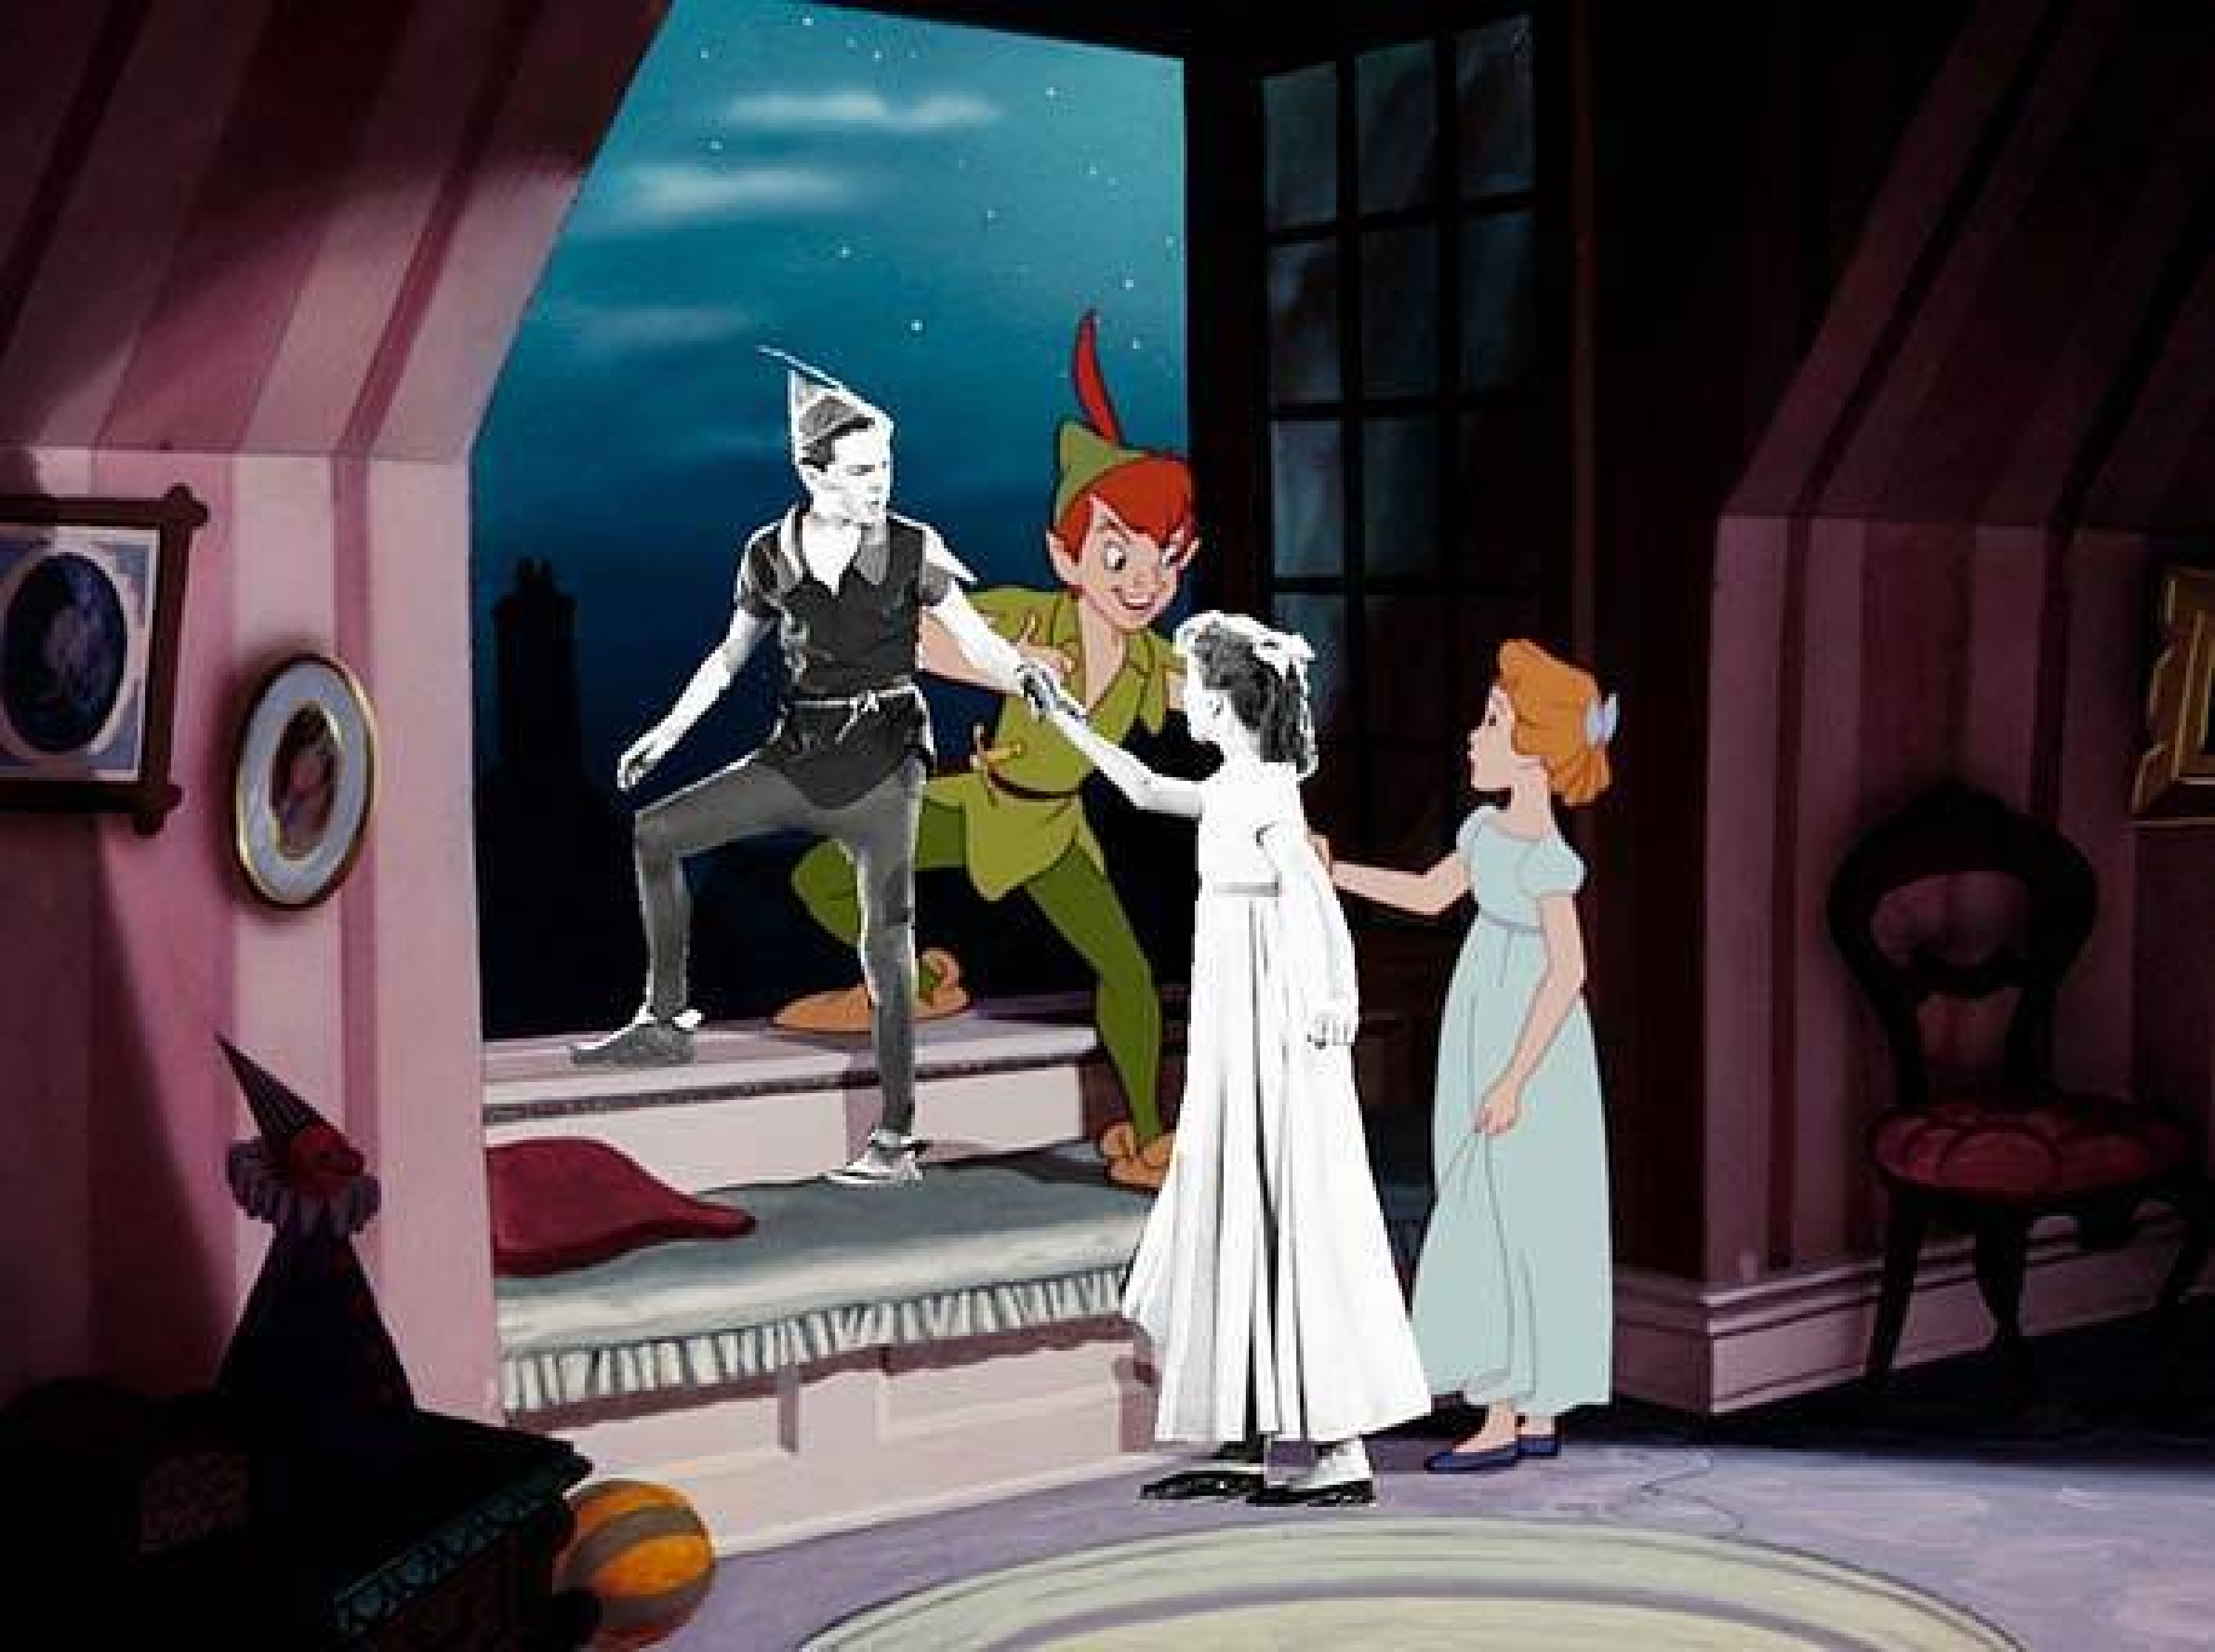
\includegraphics[width=1\linewidth]{img/relatedwork/disney_rotoscope.pdf} \\
    \caption{Rotoscoping Process for Disney's Peter Pan (1953)~\cite{peterPanRotoscoping}}
    \vspace{-15pt}
    \label{fig:disney_rotoscope}
\end{figure}

Disney's Rotoscoping Process. Disney has been known to use rotoscoping~\cite{rotoscoping} in feature films such as Snow White, Peter Pan, Sleeping Beauty, among others~\cite{rotoscopingInDisney}. This has greatly improved the quality and efficiency of their animations by not having to perform multiple cycles fo trial and error when drawing characters, adding movements, and reworking the drawings after each cycle when animating. Moreover, this also more easily captures the human gestures and expressions since the actual frames are based on real life. However, rotoscoping has had mixed reception from both animators and the art community~\cite{horrorsOfRotoscoping, tvTropesRotoscoping} due to it being completely similar to simply tracing on video and not an actual "art". In addition to this, rotoscoping limits the amount of actions animators can do compared to simply animation from imagination. This is precisely why only some aspects of the anime production process can use this method. Taking this concept, it is however possible to consider this more as an art of acting, rather than animation, and thus can be considered as a form of process speed improvement for both efficiency and speed. Complete rotoscoping has not been used in the proposed process, and only takes in motions of the 3D models moved through motion capture as a reference rather than a complete copy. The hair, clothes, and even the dynamics that all boil down to the 12 principles of animation is still applied, and this gives much more control on how the output is created. This is similar to simply using real-life models and mannequins as figure drawing reference.